% Created by tikzDevice version 0.12.3.1 on 2022-04-28 13:47:25
% !TEX encoding = UTF-8 Unicode
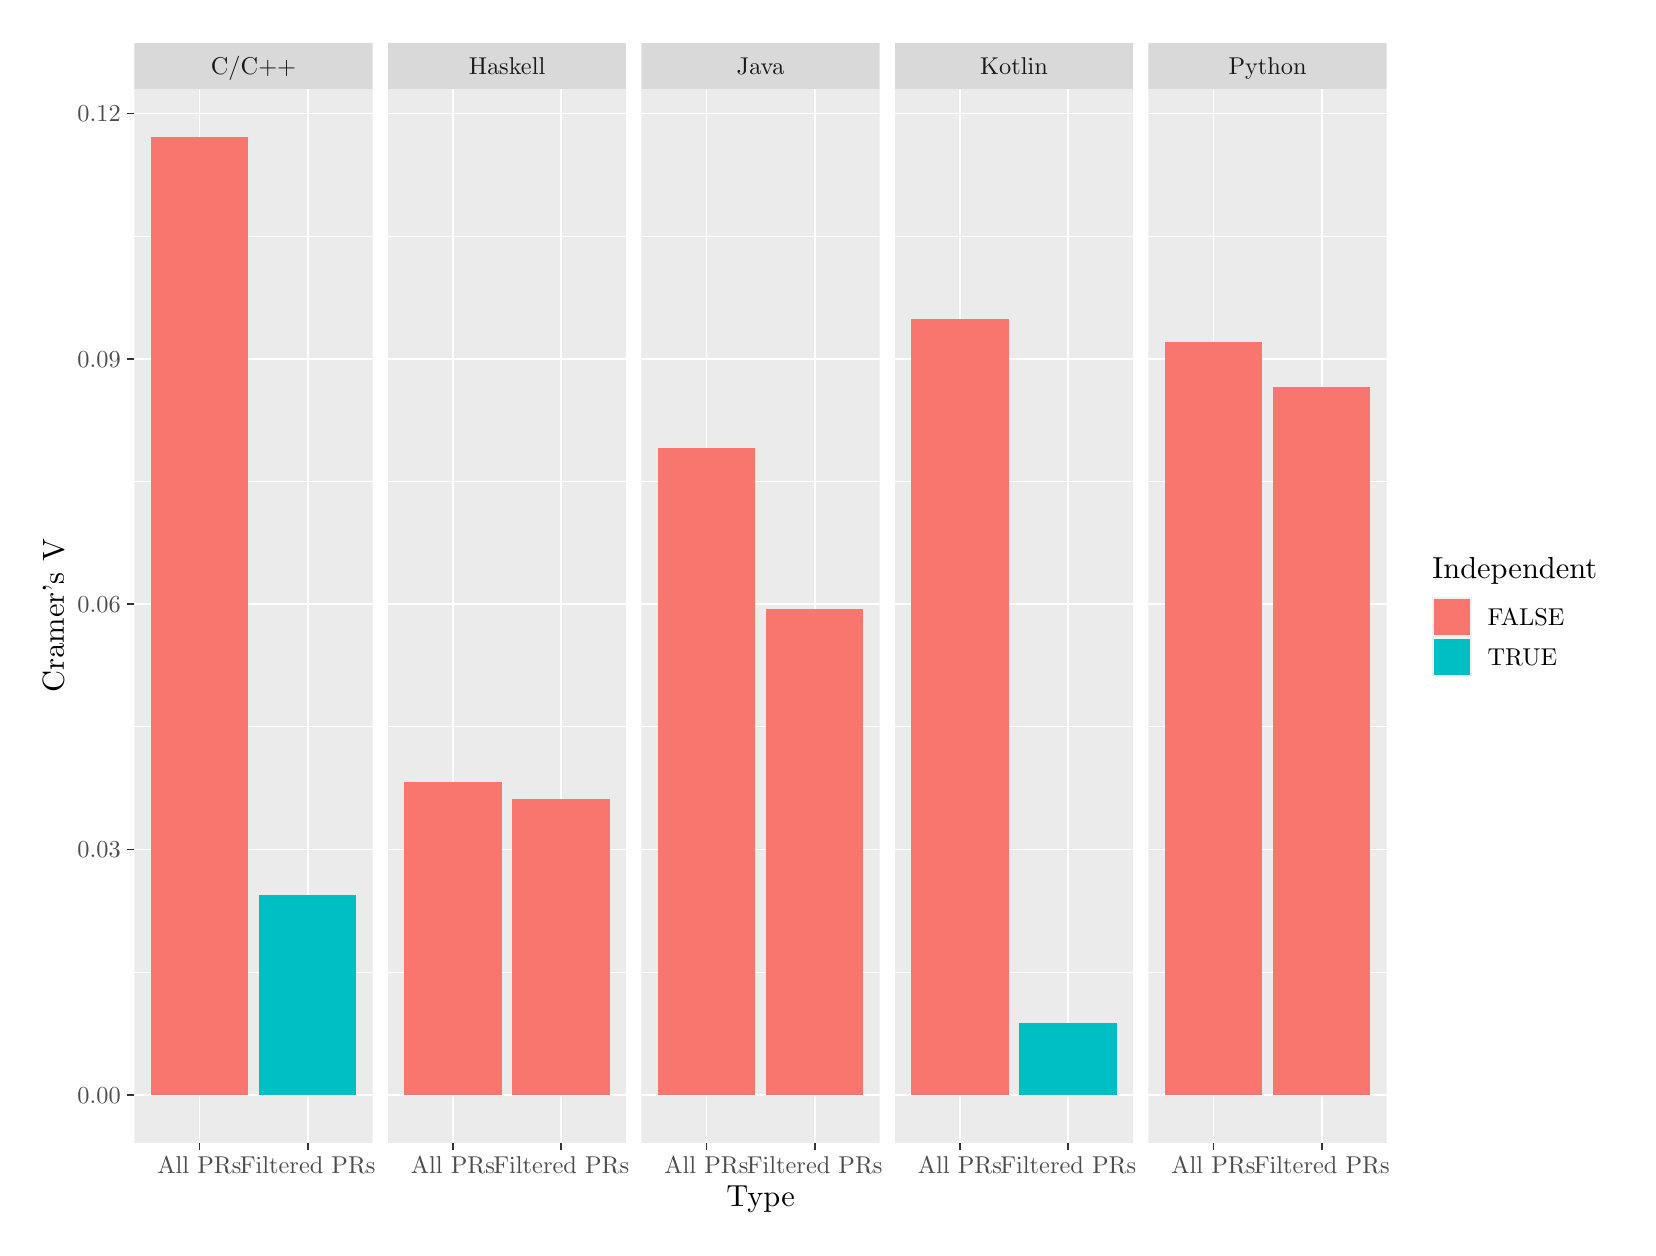
\begin{tikzpicture}[x=1pt,y=1pt]
\definecolor{fillColor}{RGB}{255,255,255}
\path[use as bounding box,fill=fillColor,fill opacity=0.00] (0,0) rectangle (578.16,433.62);
\begin{scope}
\path[clip] (  0.00,  0.00) rectangle (578.16,433.62);
\definecolor{drawColor}{RGB}{255,255,255}
\definecolor{fillColor}{RGB}{255,255,255}

\path[draw=drawColor,line width= 0.6pt,line join=round,line cap=round,fill=fillColor] (  0.00,  0.00) rectangle (578.16,433.62);
\end{scope}
\begin{scope}
\path[clip] ( 38.56, 30.69) rectangle (124.66,411.55);
\definecolor{fillColor}{gray}{0.92}

\path[fill=fillColor] ( 38.56, 30.69) rectangle (124.66,411.55);
\definecolor{drawColor}{RGB}{255,255,255}

\path[draw=drawColor,line width= 0.3pt,line join=round] ( 38.56, 92.33) --
	(124.66, 92.33);

\path[draw=drawColor,line width= 0.3pt,line join=round] ( 38.56,180.99) --
	(124.66,180.99);

\path[draw=drawColor,line width= 0.3pt,line join=round] ( 38.56,269.66) --
	(124.66,269.66);

\path[draw=drawColor,line width= 0.3pt,line join=round] ( 38.56,358.32) --
	(124.66,358.32);

\path[draw=drawColor,line width= 0.6pt,line join=round] ( 38.56, 48.00) --
	(124.66, 48.00);

\path[draw=drawColor,line width= 0.6pt,line join=round] ( 38.56,136.66) --
	(124.66,136.66);

\path[draw=drawColor,line width= 0.6pt,line join=round] ( 38.56,225.33) --
	(124.66,225.33);

\path[draw=drawColor,line width= 0.6pt,line join=round] ( 38.56,313.99) --
	(124.66,313.99);

\path[draw=drawColor,line width= 0.6pt,line join=round] ( 38.56,402.65) --
	(124.66,402.65);

\path[draw=drawColor,line width= 0.6pt,line join=round] ( 62.04, 30.69) --
	( 62.04,411.55);

\path[draw=drawColor,line width= 0.6pt,line join=round] (101.18, 30.69) --
	(101.18,411.55);
\definecolor{fillColor}{RGB}{248,118,109}

\path[fill=fillColor] ( 44.43, 48.00) rectangle ( 79.65,394.24);
\definecolor{fillColor}{RGB}{0,191,196}

\path[fill=fillColor] ( 83.57, 48.00) rectangle (118.79,120.28);
\end{scope}
\begin{scope}
\path[clip] (130.16, 30.69) rectangle (216.27,411.55);
\definecolor{fillColor}{gray}{0.92}

\path[fill=fillColor] (130.16, 30.69) rectangle (216.27,411.55);
\definecolor{drawColor}{RGB}{255,255,255}

\path[draw=drawColor,line width= 0.3pt,line join=round] (130.16, 92.33) --
	(216.27, 92.33);

\path[draw=drawColor,line width= 0.3pt,line join=round] (130.16,180.99) --
	(216.27,180.99);

\path[draw=drawColor,line width= 0.3pt,line join=round] (130.16,269.66) --
	(216.27,269.66);

\path[draw=drawColor,line width= 0.3pt,line join=round] (130.16,358.32) --
	(216.27,358.32);

\path[draw=drawColor,line width= 0.6pt,line join=round] (130.16, 48.00) --
	(216.27, 48.00);

\path[draw=drawColor,line width= 0.6pt,line join=round] (130.16,136.66) --
	(216.27,136.66);

\path[draw=drawColor,line width= 0.6pt,line join=round] (130.16,225.33) --
	(216.27,225.33);

\path[draw=drawColor,line width= 0.6pt,line join=round] (130.16,313.99) --
	(216.27,313.99);

\path[draw=drawColor,line width= 0.6pt,line join=round] (130.16,402.65) --
	(216.27,402.65);

\path[draw=drawColor,line width= 0.6pt,line join=round] (153.65, 30.69) --
	(153.65,411.55);

\path[draw=drawColor,line width= 0.6pt,line join=round] (192.79, 30.69) --
	(192.79,411.55);
\definecolor{fillColor}{RGB}{248,118,109}

\path[fill=fillColor] (136.03, 48.00) rectangle (171.26,160.99);

\path[fill=fillColor] (175.17, 48.00) rectangle (210.40,154.78);
\end{scope}
\begin{scope}
\path[clip] (221.77, 30.69) rectangle (307.88,411.55);
\definecolor{fillColor}{gray}{0.92}

\path[fill=fillColor] (221.77, 30.69) rectangle (307.88,411.55);
\definecolor{drawColor}{RGB}{255,255,255}

\path[draw=drawColor,line width= 0.3pt,line join=round] (221.77, 92.33) --
	(307.88, 92.33);

\path[draw=drawColor,line width= 0.3pt,line join=round] (221.77,180.99) --
	(307.88,180.99);

\path[draw=drawColor,line width= 0.3pt,line join=round] (221.77,269.66) --
	(307.88,269.66);

\path[draw=drawColor,line width= 0.3pt,line join=round] (221.77,358.32) --
	(307.88,358.32);

\path[draw=drawColor,line width= 0.6pt,line join=round] (221.77, 48.00) --
	(307.88, 48.00);

\path[draw=drawColor,line width= 0.6pt,line join=round] (221.77,136.66) --
	(307.88,136.66);

\path[draw=drawColor,line width= 0.6pt,line join=round] (221.77,225.33) --
	(307.88,225.33);

\path[draw=drawColor,line width= 0.6pt,line join=round] (221.77,313.99) --
	(307.88,313.99);

\path[draw=drawColor,line width= 0.6pt,line join=round] (221.77,402.65) --
	(307.88,402.65);

\path[draw=drawColor,line width= 0.6pt,line join=round] (245.25, 30.69) --
	(245.25,411.55);

\path[draw=drawColor,line width= 0.6pt,line join=round] (284.39, 30.69) --
	(284.39,411.55);
\definecolor{fillColor}{RGB}{248,118,109}

\path[fill=fillColor] (227.64, 48.00) rectangle (262.87,281.65);

\path[fill=fillColor] (266.78, 48.00) rectangle (302.01,223.44);
\end{scope}
\begin{scope}
\path[clip] (313.38, 30.69) rectangle (399.48,411.55);
\definecolor{fillColor}{gray}{0.92}

\path[fill=fillColor] (313.38, 30.69) rectangle (399.48,411.55);
\definecolor{drawColor}{RGB}{255,255,255}

\path[draw=drawColor,line width= 0.3pt,line join=round] (313.38, 92.33) --
	(399.48, 92.33);

\path[draw=drawColor,line width= 0.3pt,line join=round] (313.38,180.99) --
	(399.48,180.99);

\path[draw=drawColor,line width= 0.3pt,line join=round] (313.38,269.66) --
	(399.48,269.66);

\path[draw=drawColor,line width= 0.3pt,line join=round] (313.38,358.32) --
	(399.48,358.32);

\path[draw=drawColor,line width= 0.6pt,line join=round] (313.38, 48.00) --
	(399.48, 48.00);

\path[draw=drawColor,line width= 0.6pt,line join=round] (313.38,136.66) --
	(399.48,136.66);

\path[draw=drawColor,line width= 0.6pt,line join=round] (313.38,225.33) --
	(399.48,225.33);

\path[draw=drawColor,line width= 0.6pt,line join=round] (313.38,313.99) --
	(399.48,313.99);

\path[draw=drawColor,line width= 0.6pt,line join=round] (313.38,402.65) --
	(399.48,402.65);

\path[draw=drawColor,line width= 0.6pt,line join=round] (336.86, 30.69) --
	(336.86,411.55);

\path[draw=drawColor,line width= 0.6pt,line join=round] (376.00, 30.69) --
	(376.00,411.55);
\definecolor{fillColor}{RGB}{248,118,109}

\path[fill=fillColor] (319.25, 48.00) rectangle (354.47,328.23);
\definecolor{fillColor}{RGB}{0,191,196}

\path[fill=fillColor] (358.39, 48.00) rectangle (393.61, 73.81);
\end{scope}
\begin{scope}
\path[clip] (404.98, 30.69) rectangle (491.09,411.55);
\definecolor{fillColor}{gray}{0.92}

\path[fill=fillColor] (404.98, 30.69) rectangle (491.09,411.55);
\definecolor{drawColor}{RGB}{255,255,255}

\path[draw=drawColor,line width= 0.3pt,line join=round] (404.98, 92.33) --
	(491.09, 92.33);

\path[draw=drawColor,line width= 0.3pt,line join=round] (404.98,180.99) --
	(491.09,180.99);

\path[draw=drawColor,line width= 0.3pt,line join=round] (404.98,269.66) --
	(491.09,269.66);

\path[draw=drawColor,line width= 0.3pt,line join=round] (404.98,358.32) --
	(491.09,358.32);

\path[draw=drawColor,line width= 0.6pt,line join=round] (404.98, 48.00) --
	(491.09, 48.00);

\path[draw=drawColor,line width= 0.6pt,line join=round] (404.98,136.66) --
	(491.09,136.66);

\path[draw=drawColor,line width= 0.6pt,line join=round] (404.98,225.33) --
	(491.09,225.33);

\path[draw=drawColor,line width= 0.6pt,line join=round] (404.98,313.99) --
	(491.09,313.99);

\path[draw=drawColor,line width= 0.6pt,line join=round] (404.98,402.65) --
	(491.09,402.65);

\path[draw=drawColor,line width= 0.6pt,line join=round] (428.47, 30.69) --
	(428.47,411.55);

\path[draw=drawColor,line width= 0.6pt,line join=round] (467.61, 30.69) --
	(467.61,411.55);
\definecolor{fillColor}{RGB}{248,118,109}

\path[fill=fillColor] (410.85, 48.00) rectangle (446.08,319.92);

\path[fill=fillColor] (449.99, 48.00) rectangle (485.22,303.80);
\end{scope}
\begin{scope}
\path[clip] ( 38.56,411.55) rectangle (124.66,428.12);
\definecolor{fillColor}{gray}{0.85}

\path[fill=fillColor] ( 38.56,411.55) rectangle (124.66,428.12);
\definecolor{drawColor}{gray}{0.10}

\node[text=drawColor,anchor=base,inner sep=0pt, outer sep=0pt, scale=  0.88] at ( 81.61,416.80) {C/C++};
\end{scope}
\begin{scope}
\path[clip] (130.16,411.55) rectangle (216.27,428.12);
\definecolor{fillColor}{gray}{0.85}

\path[fill=fillColor] (130.16,411.55) rectangle (216.27,428.12);
\definecolor{drawColor}{gray}{0.10}

\node[text=drawColor,anchor=base,inner sep=0pt, outer sep=0pt, scale=  0.88] at (173.22,416.80) {Haskell};
\end{scope}
\begin{scope}
\path[clip] (221.77,411.55) rectangle (307.88,428.12);
\definecolor{fillColor}{gray}{0.85}

\path[fill=fillColor] (221.77,411.55) rectangle (307.88,428.12);
\definecolor{drawColor}{gray}{0.10}

\node[text=drawColor,anchor=base,inner sep=0pt, outer sep=0pt, scale=  0.88] at (264.82,416.80) {Java};
\end{scope}
\begin{scope}
\path[clip] (313.38,411.55) rectangle (399.48,428.12);
\definecolor{fillColor}{gray}{0.85}

\path[fill=fillColor] (313.38,411.55) rectangle (399.48,428.12);
\definecolor{drawColor}{gray}{0.10}

\node[text=drawColor,anchor=base,inner sep=0pt, outer sep=0pt, scale=  0.88] at (356.43,416.80) {Kotlin};
\end{scope}
\begin{scope}
\path[clip] (404.98,411.55) rectangle (491.09,428.12);
\definecolor{fillColor}{gray}{0.85}

\path[fill=fillColor] (404.98,411.55) rectangle (491.09,428.12);
\definecolor{drawColor}{gray}{0.10}

\node[text=drawColor,anchor=base,inner sep=0pt, outer sep=0pt, scale=  0.88] at (448.04,416.80) {Python};
\end{scope}
\begin{scope}
\path[clip] (  0.00,  0.00) rectangle (578.16,433.62);
\definecolor{drawColor}{gray}{0.20}

\path[draw=drawColor,line width= 0.6pt,line join=round] ( 62.04, 27.94) --
	( 62.04, 30.69);

\path[draw=drawColor,line width= 0.6pt,line join=round] (101.18, 27.94) --
	(101.18, 30.69);
\end{scope}
\begin{scope}
\path[clip] (  0.00,  0.00) rectangle (578.16,433.62);
\definecolor{drawColor}{gray}{0.30}

\node[text=drawColor,anchor=base,inner sep=0pt, outer sep=0pt, scale=  0.88] at ( 62.04, 19.68) {All PRs};

\node[text=drawColor,anchor=base,inner sep=0pt, outer sep=0pt, scale=  0.88] at (101.18, 19.68) {Filtered PRs};
\end{scope}
\begin{scope}
\path[clip] (  0.00,  0.00) rectangle (578.16,433.62);
\definecolor{drawColor}{gray}{0.20}

\path[draw=drawColor,line width= 0.6pt,line join=round] (153.65, 27.94) --
	(153.65, 30.69);

\path[draw=drawColor,line width= 0.6pt,line join=round] (192.79, 27.94) --
	(192.79, 30.69);
\end{scope}
\begin{scope}
\path[clip] (  0.00,  0.00) rectangle (578.16,433.62);
\definecolor{drawColor}{gray}{0.30}

\node[text=drawColor,anchor=base,inner sep=0pt, outer sep=0pt, scale=  0.88] at (153.65, 19.68) {All PRs};

\node[text=drawColor,anchor=base,inner sep=0pt, outer sep=0pt, scale=  0.88] at (192.79, 19.68) {Filtered PRs};
\end{scope}
\begin{scope}
\path[clip] (  0.00,  0.00) rectangle (578.16,433.62);
\definecolor{drawColor}{gray}{0.20}

\path[draw=drawColor,line width= 0.6pt,line join=round] (245.25, 27.94) --
	(245.25, 30.69);

\path[draw=drawColor,line width= 0.6pt,line join=round] (284.39, 27.94) --
	(284.39, 30.69);
\end{scope}
\begin{scope}
\path[clip] (  0.00,  0.00) rectangle (578.16,433.62);
\definecolor{drawColor}{gray}{0.30}

\node[text=drawColor,anchor=base,inner sep=0pt, outer sep=0pt, scale=  0.88] at (245.25, 19.68) {All PRs};

\node[text=drawColor,anchor=base,inner sep=0pt, outer sep=0pt, scale=  0.88] at (284.39, 19.68) {Filtered PRs};
\end{scope}
\begin{scope}
\path[clip] (  0.00,  0.00) rectangle (578.16,433.62);
\definecolor{drawColor}{gray}{0.20}

\path[draw=drawColor,line width= 0.6pt,line join=round] (336.86, 27.94) --
	(336.86, 30.69);

\path[draw=drawColor,line width= 0.6pt,line join=round] (376.00, 27.94) --
	(376.00, 30.69);
\end{scope}
\begin{scope}
\path[clip] (  0.00,  0.00) rectangle (578.16,433.62);
\definecolor{drawColor}{gray}{0.30}

\node[text=drawColor,anchor=base,inner sep=0pt, outer sep=0pt, scale=  0.88] at (336.86, 19.68) {All PRs};

\node[text=drawColor,anchor=base,inner sep=0pt, outer sep=0pt, scale=  0.88] at (376.00, 19.68) {Filtered PRs};
\end{scope}
\begin{scope}
\path[clip] (  0.00,  0.00) rectangle (578.16,433.62);
\definecolor{drawColor}{gray}{0.20}

\path[draw=drawColor,line width= 0.6pt,line join=round] (428.47, 27.94) --
	(428.47, 30.69);

\path[draw=drawColor,line width= 0.6pt,line join=round] (467.61, 27.94) --
	(467.61, 30.69);
\end{scope}
\begin{scope}
\path[clip] (  0.00,  0.00) rectangle (578.16,433.62);
\definecolor{drawColor}{gray}{0.30}

\node[text=drawColor,anchor=base,inner sep=0pt, outer sep=0pt, scale=  0.88] at (428.47, 19.68) {All PRs};

\node[text=drawColor,anchor=base,inner sep=0pt, outer sep=0pt, scale=  0.88] at (467.61, 19.68) {Filtered PRs};
\end{scope}
\begin{scope}
\path[clip] (  0.00,  0.00) rectangle (578.16,433.62);
\definecolor{drawColor}{gray}{0.30}

\node[text=drawColor,anchor=base east,inner sep=0pt, outer sep=0pt, scale=  0.88] at ( 33.61, 44.97) {0.00};

\node[text=drawColor,anchor=base east,inner sep=0pt, outer sep=0pt, scale=  0.88] at ( 33.61,133.63) {0.03};

\node[text=drawColor,anchor=base east,inner sep=0pt, outer sep=0pt, scale=  0.88] at ( 33.61,222.30) {0.06};

\node[text=drawColor,anchor=base east,inner sep=0pt, outer sep=0pt, scale=  0.88] at ( 33.61,310.96) {0.09};

\node[text=drawColor,anchor=base east,inner sep=0pt, outer sep=0pt, scale=  0.88] at ( 33.61,399.62) {0.12};
\end{scope}
\begin{scope}
\path[clip] (  0.00,  0.00) rectangle (578.16,433.62);
\definecolor{drawColor}{gray}{0.20}

\path[draw=drawColor,line width= 0.6pt,line join=round] ( 35.81, 48.00) --
	( 38.56, 48.00);

\path[draw=drawColor,line width= 0.6pt,line join=round] ( 35.81,136.66) --
	( 38.56,136.66);

\path[draw=drawColor,line width= 0.6pt,line join=round] ( 35.81,225.33) --
	( 38.56,225.33);

\path[draw=drawColor,line width= 0.6pt,line join=round] ( 35.81,313.99) --
	( 38.56,313.99);

\path[draw=drawColor,line width= 0.6pt,line join=round] ( 35.81,402.65) --
	( 38.56,402.65);
\end{scope}
\begin{scope}
\path[clip] (  0.00,  0.00) rectangle (578.16,433.62);
\definecolor{drawColor}{RGB}{0,0,0}

\node[text=drawColor,anchor=base,inner sep=0pt, outer sep=0pt, scale=  1.10] at (264.82,  7.64) {Type};
\end{scope}
\begin{scope}
\path[clip] (  0.00,  0.00) rectangle (578.16,433.62);
\definecolor{drawColor}{RGB}{0,0,0}

\node[text=drawColor,rotate= 90.00,anchor=base,inner sep=0pt, outer sep=0pt, scale=  1.10] at ( 13.08,221.12) {Cramer's V};
\end{scope}
\begin{scope}
\path[clip] (  0.00,  0.00) rectangle (578.16,433.62);
\definecolor{fillColor}{RGB}{255,255,255}

\path[fill=fillColor] (502.09,193.56) rectangle (572.66,248.68);
\end{scope}
\begin{scope}
\path[clip] (  0.00,  0.00) rectangle (578.16,433.62);
\definecolor{drawColor}{RGB}{0,0,0}

\node[text=drawColor,anchor=base west,inner sep=0pt, outer sep=0pt, scale=  1.10] at (507.59,234.53) {Independent};
\end{scope}
\begin{scope}
\path[clip] (  0.00,  0.00) rectangle (578.16,433.62);
\definecolor{fillColor}{gray}{0.95}

\path[fill=fillColor] (507.59,213.51) rectangle (522.04,227.96);
\end{scope}
\begin{scope}
\path[clip] (  0.00,  0.00) rectangle (578.16,433.62);
\definecolor{fillColor}{RGB}{248,118,109}

\path[fill=fillColor] (508.30,214.22) rectangle (521.33,227.25);
\end{scope}
\begin{scope}
\path[clip] (  0.00,  0.00) rectangle (578.16,433.62);
\definecolor{fillColor}{gray}{0.95}

\path[fill=fillColor] (507.59,199.06) rectangle (522.04,213.51);
\end{scope}
\begin{scope}
\path[clip] (  0.00,  0.00) rectangle (578.16,433.62);
\definecolor{fillColor}{RGB}{0,191,196}

\path[fill=fillColor] (508.30,199.77) rectangle (521.33,212.80);
\end{scope}
\begin{scope}
\path[clip] (  0.00,  0.00) rectangle (578.16,433.62);
\definecolor{drawColor}{RGB}{0,0,0}

\node[text=drawColor,anchor=base west,inner sep=0pt, outer sep=0pt, scale=  0.88] at (527.54,217.71) {FALSE};
\end{scope}
\begin{scope}
\path[clip] (  0.00,  0.00) rectangle (578.16,433.62);
\definecolor{drawColor}{RGB}{0,0,0}

\node[text=drawColor,anchor=base west,inner sep=0pt, outer sep=0pt, scale=  0.88] at (527.54,203.25) {TRUE};
\end{scope}
\end{tikzpicture}
